\newpage
\usecasebase{Visualizzazione del riepilogo prenotazione}
\label{usecase:Visualizzazione del riepilogo prenotazione}

\begin{figure}[h]
	\centering
	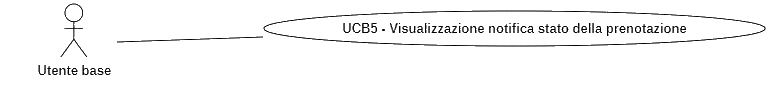
\includegraphics[width=0.8\textwidth]{./uml/UCB5.png} 
	\caption{Visualizzazione del riepilogo prenotazione}
	\label{fig:UCB5}
  \end{figure}

\begin{itemize}
	\item \textbf{Descrizione:}
	Il riepilogo della prenotazione include almeno i seguenti campi:
	\begin{itemize}
		\item \textbf{Nome ristorante:} Denominazione del ristorante.
		\item \textbf{Data e ora:} Data e ora della prenotazione.
		\item \textbf{Numero di persone:} Numero di persone coinvolte nella prenotazione.
		\item \textbf{\textit{Username}:} \textit{Username} dell'Utente base associato alla prenotazione o lista degli \textit{username} degli Utenti base associati.

		\item \textbf{Stato$^G$:} Stato della prenotazione, che può essere uno tra i seguenti:
			  \begin{itemize}
				  \item \textbf{In attesa:} la prenotazione è in attesa di accettazione da parte del ristorante.
				  \item \textbf{Accettata:} la prenotazione è stata accettata dal ristorante.
				  \item \textbf{Rifiutata:} la prenotazione è stata rifiutata dal ristorante.
				  \item \textbf{In corso:} la prenotazione è attualmente in corso.
				  \item \textbf{Terminata:} la prenotazione è terminata e il conto è stato pagato.
				  \item \textbf{Annullata:} la prenotazione è stata annullata.
			  \end{itemize}
	\end{itemize}
	
	\item \textbf{Attore principale:} Utente base.

	\item \textbf{Precondizioni:}
	      \begin{itemize}
		      \item L'Utente sta visualizzando la lista di tutte le sue prenotazioni (vedi \autoref{usecase:Visualizzazione lista delle prenotazioni}).
		      \item L'Utente base ha precedentemente effettuato una prenotazione (vedi \autoref{usecase:Prenotazione di un tavolo}).
	      \end{itemize}


	\item \textbf{Postcondizione:}
	      L'Utente base visualizza in dettaglio il riepilogo di una sua prenotazione.

	\item \textbf{Scenario principale:}
	      \begin{enumerate}
		      \item L'Utente base visualizza il riepilogo della prenotazione e le sue informazioni;
		      \item Il Sistema mostra il riepilogo della prenotazione e le relative informazioni (vedi \textbf{Descrizione}).
	      \end{enumerate}
\end{itemize}
